\chapter{Implementation}
\label{chapter3}

This chapter will go through the implementation of the project. First, the system information and general program structure will be looked at. Then, the rendering of fractals will be covered, followed by the attempts at improving performance, and the method of measuring performance. Finally, there will be a section on debugging.\newline

In terms of general optimizations, there were no specific efforts to optimize the code or the basic algorithms (except perhaps to implement a view distance limit), since the most important thing was to remain consistent across the different scenarios, and the relevant measurements were the performance differences (if any), not the raw performance.

\section{Operating System and Hardware}

The operating system used was Linux Mint 20.1. The project compiles on Linux using Make. Considering that the project was written in C, it is likely very portable (as long as the system can use Vulkan as well), but compilation on other operating systems has not been tested, and would require changes to the method of compilation.\newline

The CPU used was an Intel\copyright Core$^{TM}$ i7-9750H with 6 cores.

The GPU used was an NVIDIA TU106M (GeForce RTX 2060 Mobile).

The Vulkan version being used was 1.3.205.

\section{Program Structure and Libraries}

\subsection{Libraries Used}

\subsubsection{Vulkan}

Vulkan was chosen over OpenGL because it is performant and modern, and because there are some changes on the way that will, I think, help with the efficiency of rendering using one of the optimization methods chosen (though it is not supported currently, unfortunately). Additionally, it seemed like the logical choice, as I am at the moment more familiar with Vulkan than with OpenGL and have, as of writing this, worked with it more recently. It is licensed under the Apache License 2.0 \cite{licensing-vulkan}.

\subsubsection{Volk}

The third-party library, Volk, is a meta-loader for Vulkan. It allows one to load the Vulkan API without needing to link to Vulkan. This makes setup much easier to manage. It is licensed under the MIT license \cite{licensing-volk}.

\subsubsection{GLFW}

GLFW is a library for creating windows and surfaces, which can be used for Vulkan development. It is easy to use and multi-platform, and written in C, so is the logical choice for this project. It is licensed under the zlib/libpng license \cite{licensing-glfw}.

\subsection{Programming Language}

The programming language of choice for this project was C. C was chosen because it is the language that the libraries used (Vulkan and GLFW) were written in. It was chosen over C++, because the usual desirable additional features, such as vectors, were not needed, so memory management was easy.\newline

Using C over C++, some additional complexity was added due to Vulkan objects needing explicit destruction. In C++, it's possible to use the destructors of classes to handle this automatically. However, a pattern for destroying Vulkan objects was established, and did not add much extra work.\newline

GLM is a library in C++, often used for handling matrix and vector operations. For this project, there was comparatively little need for such operations, when compared to a program that renders pre-calculated or stored geometry such as meshes, so a very lightweight set of functions was written for the few vector operations that were needed (and no matrix operations at all).\newline

Overall, the project was intended to be lightweight and simple, and it was decided that using C was the best choice, and that using C++ would not significantly reduce complexity. C++ is certainly worth using if dynamic data structures like vectors are needed, or explicit memory management would add a lot of complexity to the code. In this project, that was not the case.

\subsection{Vulkan Setup}

The project used Vulkan for rendering. The rendering process was split into two passes, one for geometry and one for colour. This was done because the speed at which the geometry of the scene was obtained was of interest, and the speed of colouring the fractals was not, so splitting them enabled measurement of the geometry render pass on its own.\newline

No vertices are passed in to the shaders; the vertex shaders conjure up fullscreen triangles using the vertex indices, which are then worked on by the fragment shaders, where all the calculations and colouring happen.\newline

Specific setups for different optimization methods will be discussed in the relevant sections.

\subsection{Program Layout}

The program takes arguments which specify the setup when the program is loaded. The user can change which fractal to display (including the 2D Mandelbrot set, the Mandelbulb and the Hall of Pillars), which optimization method to use, whether to vary any fractal parameters (which can be used to animate the fractal) and whether to take any performance measurements during runtime. Some of the arguments affect which shaders are loaded, and the Vulkan setup.\newline

The user is able to control the camera with the mouse and keyboard, speed up and slow down, and print the current position and camera front vector. Input is handled by GLFW.

\section{Rendering 3D Fractals}

The project made use of two fractal formulae. One was for the Mandelbulb, as described in the background section. Another was chosen to provide variety, specifically with regards to the depth of the image. The Mandelbulb is neatly contained within a box, and has no "interior", but the alternative fractal (named "Hall of Pillars" by me given its lack of another name) takes up the entire screen, and is reminiscent of a room with many archways, which I thought might give different results in terms of the performance measurements when using the optimizations developed in the project.\newline

The calculations for the fractals were done entirely within shaders, except for the generation of the 3D signed distance field, which was calculated on the CPU upon loading the program, before any rendering occurred. Single-precision floating point numbers were used for all calculations within shaders. These were chosen over double-precision numbers, as the scale of the fractals was reasonable, and high-detail zooms into the fractal were not necessary for the project.

\subsection{Basic Sphere Tracing Implementation}

The basic sphere tracing algorithm was implemented in GLSL and is largely the same across the fractal types and optimization methods. Figure \ref{figure:glsl-sphere-tracing} below shows the implementation.

\begin{figure}[ht]
	\centering
	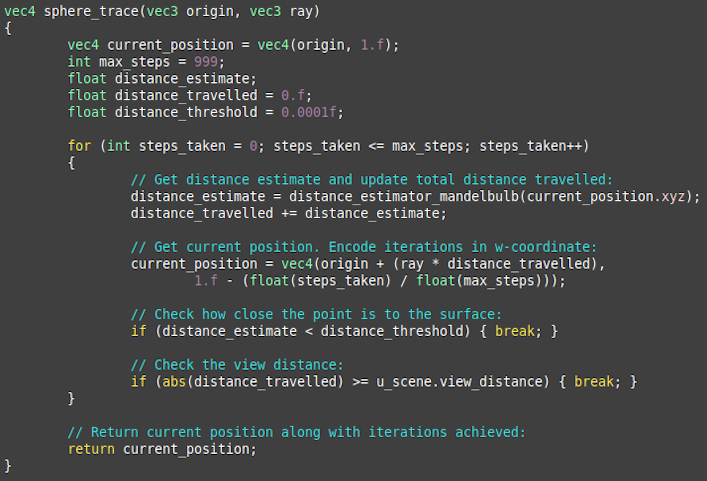
\includegraphics[width=0.65\linewidth, frame]{Images/GLSL-Sphere-Tracing.png}
	\caption{GLSL code snippet of the sphere tracing algorithm.}
	\label{figure:glsl-sphere-tracing}
\end{figure}

The most important things that must remain consistent between different optimizations on the same fractal are the termination conditions, which are as follows:

\begin{itemize}
	\item The maximum number of iterations allowed.
	\item The distance threshold.
	\item The view distance, contained in the scene uniform.
\end{itemize}

\subsection{Mandelbulb Fractal}

\begin{figure}[ht]
	\centering
	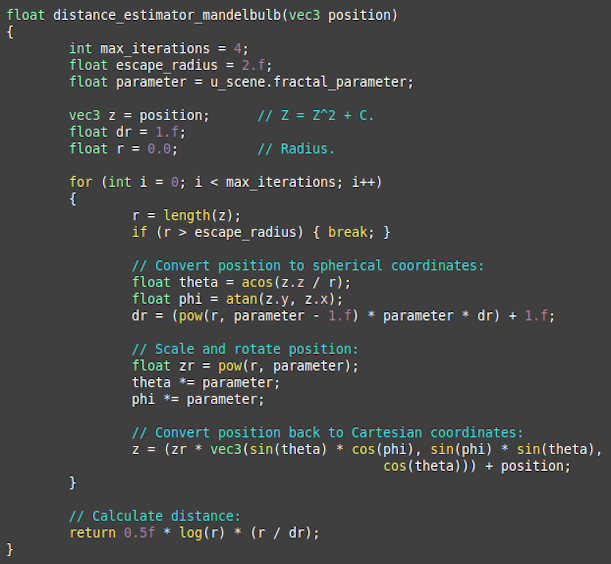
\includegraphics[width=0.65\linewidth, frame]{Images/GLSL-Distance-Estimator-Mandelbulb.png}
	\caption{GLSL code snippet of the distance estimator function for the Mandelbulb fractal.}
	\label{figure:glsl-distance-estimator-mandelbulb}
\end{figure}

Shader implementation of signed distance function for Mandelbulb

View distance limit

\subsection{Alternative Fractal}

\begin{figure}[ht]
	\centering
	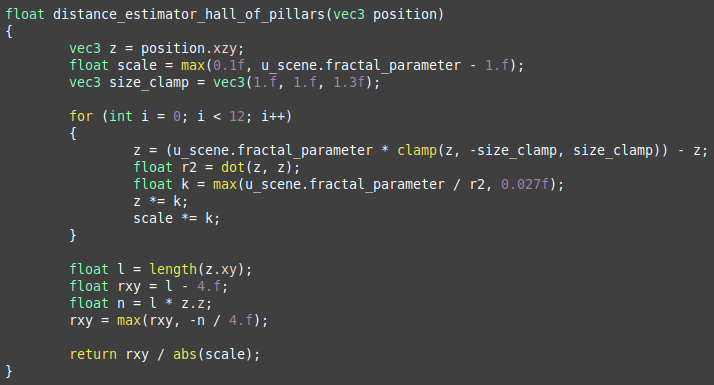
\includegraphics[width=0.65\linewidth, frame]{Images/GLSL-Distance-Estimator-Hall-Of-Pillars.png}
	\caption{GLSL code snippet of the distance estimator function for the alternative "Hall of Pillars" fractal. Credit goes to Dave Hoskins for the formula \cite{shadertoy-hall-of-pillars}.}
	\label{figure:glsl-distance-estimator-hall-of-pillars}
\end{figure}



Got fractal shader code from Shadertoy (link, mention license), have named it "Hall of Pillars". Show signed distance function shader.

View distance limit is higher because fractal is bigger.

\subsection{Colour, Ambient Occlusion and Fog}

Be very brief here, colour isn't important. Fog is for graceful cutoff of view instead of sharp drop.

Number of iterations is good in this case for viewing performance differences, but also for ambient occlusion. So it is combined with the colour.

Number of iterations is raised to a power, since the number of iterations allowed is very high (999). Raising it to a power amplifies the differences. This is done consistently so won't affect comparison of images, but will make it easier and more visible.

\section{3D Signed Distance Field}

Centered around fractal - Mandelbulb

Centered around camera - Hall of Pillars?

\section{Temporal Caching}

Single image - memory of 4 previous frames.

Why did I choose length / 4? Be more scientific about it.

Talk about how you dealt with movement - temporal reprojection? Wanted to deal with the specific scenario where the distance recorded is greater than the true distance. My method relies on the landscape not being smooth, so these changes happen often. Maybe find another method.

\section{Performance Measurement}

\subsection{Data Types Collected}

Mention image copying time and how it could be avoided altogether, so didn't measure.

Measured geometry pass time.

Median, min, max, frame time.

\subsection{Representative Views}

Hall of Pillars - Room with archway

Hall of Pillars - Flat ground

Hall of Pillars - Room with huge distance differences and bottlenecks

Hall of Pillars - Room with very short distance to back, maybe bottlenecks

Mandelbulb - Full view, lots of white space

Mandelbulb - Zoomed in so it covers the screen

Mandelbulb - Try to find a view with bottleneck

Mandelbulb - Zoom in to get detail

\subsection{Animation}

Hall of Pillars - Flythrough

Hall of Pillars - Varying parameter?

Mandelbulb - Varying parameter

Mandelbulb - Fly across? Probably not.

\section{Debugging and Optimization}

Manual debugging - printing out Vulkan handles, error handling with messages, printing current position/rotation, using Renderdoc to view different pipeline stages to make sure they are coming out correctly. Adding special return values in shaders to output black if something has not gone right.

No extra optimization has been done, since the project is focused on performance difference between methods, not on raw performance numbers. Therefore, optimizations such as early ray culling (the Mandelbulb fractal, for example, is contained more or less within a cube with side lengths of 2.2) have not been implemented.